\section{Теоретическая часть}

\begin{figure}[h]
	\centering
	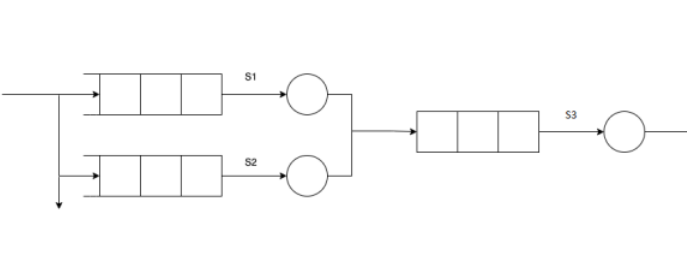
\includegraphics[width=0.7\linewidth]{src/Снимок}
	\caption{}
	\label{fig:}
\end{figure}

\begin{figure}[h]
	\centering
	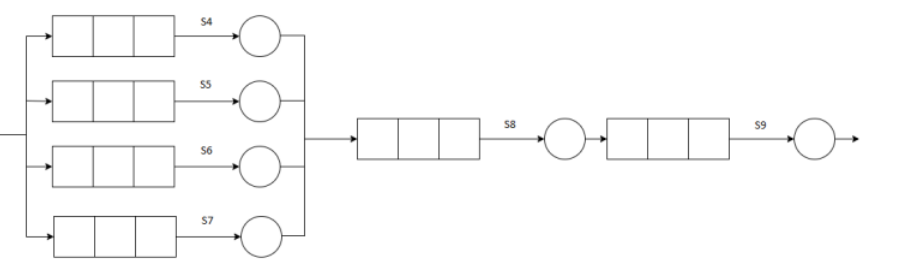
\includegraphics[width=0.7\linewidth]{src/Снимок1}
	\caption{}
	\label{fig:1}
\end{figure}

\begin{enumerate}
	\item S1, S2 – операторы;
	\item S3 – приём техники на починку;
	\item S4, S5, S6, S7 – восстановительные работы;
	\item S8 – отправка техники;
	\item S9 – выдача.
\end{enumerate}






